\documentclass{tufte-handout}

\title{CS294: Deep Reinforcement Learning
       \thanks{Course Instructors: Sergey Levine} \\
       \Large Lecture Notes: Value Functions Introduction \thanks{Author: InnerPeace}}

\date{Fall 2017\thanks{Un-official Lecture Notes}} % without \date command, current date is supplied

%\geometry{showframe} % display margins for debugging page layout

\usepackage{graphicx} % allow embedded images
  \setkeys{Gin}{width=\linewidth,totalheight=\textheight,keepaspectratio}
  \graphicspath{{notes5/fig/}} % set of paths to search for images
\usepackage{amsmath}  % extended mathematics
\usepackage{amstext}  % extended text
\usepackage{booktabs} % book-quality tables
\usepackage{units}    % non-stacked fractions and better unit spacing
\usepackage{multicol} % multiple column layout facilities
\usepackage{lipsum}   % filler text
\usepackage{cancel}
\usepackage{algorithm}
\usepackage{algorithmic}
\usepackage{fancyvrb} % extended verbatim environments
\usepackage{placeins}
  \fvset{fontsize=\normalsize}% default font size for fancy-verbatim environments
\usepackage[normalem]{ulem}
% \usepackage{algpseudocode}
% \usepackage{algorithm}


% tikz package
\usepackage{tikz}
\usetikzlibrary{patterns, shapes,calc,positioning,arrows,mindmap,matrix}
\usetikzlibrary{decorations.pathreplacing}

% Standardize command font styles and environments
\newcommand{\doccmd}[1]{\texttt{\textbackslash#1}}% command name -- adds backslash automatically
\newcommand{\docopt}[1]{\ensuremath{\langle}\textrm{\textit{#1}}\ensuremath{\rangle}}% optional command argument
\newcommand{\docarg}[1]{\textrm{\textit{#1}}}% (required) command argument
\newcommand{\docenv}[1]{\textsf{#1}}% environment name
\newcommand{\docpkg}[1]{\texttt{#1}}% package name
\newcommand{\doccls}[1]{\texttt{#1}}% document class name
\newcommand{\docclsopt}[1]{\texttt{#1}}% document class option name
\newenvironment{docspec}{\begin{quote}\noindent}{\end{quote}}% command specification environment
\newcommand{\argmin}{\operatornamewithlimits{argmin}}
\newcommand{\argmax}{\operatornamewithlimits{argmax}}
\newcommand{\textunderscript}[1]{$_{\text{#1}}$}

\newcommand{\etal}{\textit{et al}. }
\newcommand{\ie}{\textit{i}.\textit{e}., }
\newcommand{\eg}{\textit{e}.\textit{g}. }
\newcommand{\s}{\mathbf{s}}
\newcommand{\act}{\mathbf{a}}
\newcommand{\wrt}{\textit{w}.\textit{r}.\textit{t}. }

\setcounter{secnumdepth}{3}

\begin{document}

\maketitle% this prints the handout title, author, and date

\textbf{Keyphrases: Value Function. Advantage Function. Q-learning. Policy Iteration. }\\

\noindent{}This set of notes introduces the idea of improving policy only by using a critic, without an actor. We then discuss how to extract policy from a value function. Lastly, we will introduce the \emph{Q-learning} algorithm, how it works and practical considerations.

\section{Policy Iteration}

We learned that \emph{policy gradient} is intuitive and closely related to the usual supervised learning algorithms we are familiar with, but it's noisy
and has high variance. Can we find a way to get rid of it? In \emph{actor-critic}, we estimated the advantage function $\hat{A}^\pi(\s_t, \act_t)$
which represents how much better is $\act_t$ than the average action according to $\pi$. It turns out that advantage function is quiet useful, cause we can
find out the \emph{best} action from $\s_t$ following $\pi$ afterwards, which is $\arg \max_{\act_t} \hat{A}^\pi(\s_t, \act_t)$. And if we can find out the
best action at every time-step, we can improve the policy with the mechanism, then problem's solved regardless of what the policy is. Besides, with this idea, we use only the advantage function without worrying about the high variance sort of problems of policy gradient.

\begin{marginfigure}
\centering
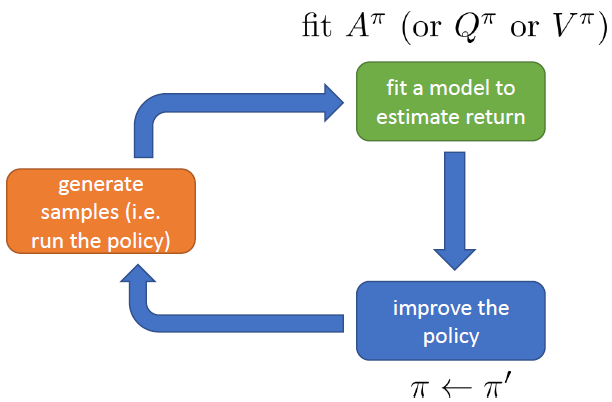
\includegraphics[width=\linewidth]{intro}
\caption{General scheme of improving policy with advantage.}
\label{fig:intro}
\end{marginfigure}

The resulting mechanism is straightforward. The new policy assigns the probability 1 to the best action at that time-step and 0 to other actions. And the new policy is at least as good as $\pi$, then we can improve policy with this mechanism iteratively.

\begin{equation}
\label{eq:1}
\pi'(\act_t | \s_t) = \begin{cases}
1 \quad \text{if} \; \act_t = \arg \max_{\act_t} \hat{A}^\pi(\s_t, \act_t) \\
0 \quad \text{otherwise}
\end{cases}
\end{equation}

\begin{algorithm}
  \caption{Policy Iteration Algorithm}
    \label{algo:policyiter}
    \begin{algorithmic}[1]
    % \REQUIRE some words.  % this command shows "Input"
    % \ENSURE
    \WHILE {\emph{Not converged}}
    \STATE Evaluate $\hat{A} ^\pi(\s, \act)$. \\
    \STATE Update $ \pi \leftarrow \pi'$. \\
    \ENDWHILE
    \RETURN improved policy $\pi$  % this command shows "Output"
  \end{algorithmic}
\end{algorithm}

The way to evaluate $\hat{A} ^\pi(\s, \act)$ is the same as \emph{actor-critic} where

\begin{equation}
\label{eq:2}
A^\pi (\s, \act) = r(\s, \act) + \gamma E[V^\pi(\s')] - V^\pi(\s)
\end{equation}

And we only need to evaluate $V^\pi$ during iteration.

\subsection{Dynamic Programming}

To elaborate this idea, we start with a toy example assuming that we know the dynamic, and state and action are both discrete and small. Suppose that we are
in a grid world which has the size of $4 \; \times \; 4$ (figure \ref{fig:grid}) with 16 states and 4 actions per state by walking to different directions. We can store full $V^\pi (\s)$ in a table.

\begin{marginfigure}
\centering
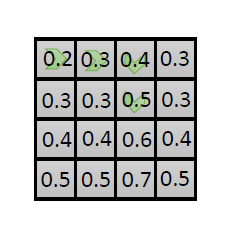
\includegraphics[width=\linewidth]{grid}
\caption{Tabular case which has no approximation errors w.r.t the value function.}
\label{fig:grid}
\end{marginfigure}

As for the value estimation, we discussed the \emph{bootstrapped} mode in actor-critic, where the reward plus next value is the estimation of value function, and the expectation over actions of that is the value of current state.

\begin{equation}
\label{eq:3}
V^\pi(\s) \leftarrow E_{\act \sim \pi(\act | \s)} \big[ r(\s, \act) + \gamma E_{\s' \sim p(\s' | \s, \act)} \big[V^\pi (\s') \big] \big]
\end{equation}

From equation \ref{eq:1}, only one action (best one) has non-zero probability which means that the policy $\pi$ is deterministic $\pi(\s) = \act$. Then we can simplify equation \ref{eq:3} to

\begin{equation}
\label{eq:4}
V^\pi(\s) \leftarrow  r(\s, \pi(\s)) + \gamma E_{\s' \sim p(\s' | \s, \pi(\s))} \big[V^\pi (\s') \big] \big]
\end{equation}

For the tabular case, there is no approximation errors for the estimation of $V^\pi(\s)$.

\section{Value Iteration}

The Q-function measures the expected future rewards by taking action $\act_t$ and state $\s_t$, and the relationship between Q-function and value function is:

\begin{equation}
\label{eq:5}
Q^\pi (\s, \act) = r(\s, \act) +\gamma E[V^\pi(\s')]
\end{equation}
\begin{equation}
\label{eq:6}
V^\pi (\s) = E_{\act \sim \pi(\act | \s)} [Q(\s, \act)]
\end{equation}

Interestingly, it turns out the best action w.r.t to advantage is the same as that of Q-function.

\begin{equation}
\label{eq:7}
\arg \max_{\act_t} A^\pi(\s_t, \act_t) = \arg \max_{\act_t} Q^\pi(\s_t, \act_t)
\end{equation}

\begin{marginfigure}
\centering
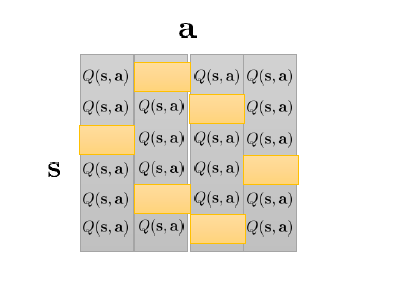
\includegraphics[width=\linewidth]{tabular-q}
\caption{Q values for tabular case, the yellow block means the biggest Q value for the each state.}
\label{fig:tabular-q}
\end{marginfigure}

Then we can replace advantage with Q-function to make it simpler for evaluating. For the tabular case, we can write out all the $Q(\s, \act)$ w.r.t every pair of state-action, and for every state, we just take the actions with biggest $Q$ which is combined to form the policy. Besides, only $\arg \max_{\act_t} Q^\pi(\s_t, \act_t)$ has probability of 1 and together with equation \ref{eq:6} we obtain that:

\begin{equation}
\label{eq:8}
V^\pi (\s) = \max_\act Q(\s, \act)
\end{equation}

Then we skip the policy and compute values directly. Finally, if we know how to represent value function $V^\pi(\s)$, then together with those ideas, it forms the \emph{value iteration algorithm}.

\begin{algorithm}
  \caption{Value Iteration Algorithm}
    \label{algo:value-iter}
    \begin{algorithmic}[1]
    % \REQUIRE some words.  % this command shows "Input"
    % \ENSURE
    \WHILE {\emph{Not converged}}
    \STATE Evaluate $Q^\pi (\s, \act) = r(\s, \act) +\gamma E[V^\pi(\s')]$. \\
    \STATE Update $ V^\pi (\s) = \max_\act Q(\s, \act)$. \\
    \ENDWHILE
    % \RETURN improved policy $\pi$  % this command shows "Output"
  \end{algorithmic}
\end{algorithm}

\begin{marginfigure}
\centering
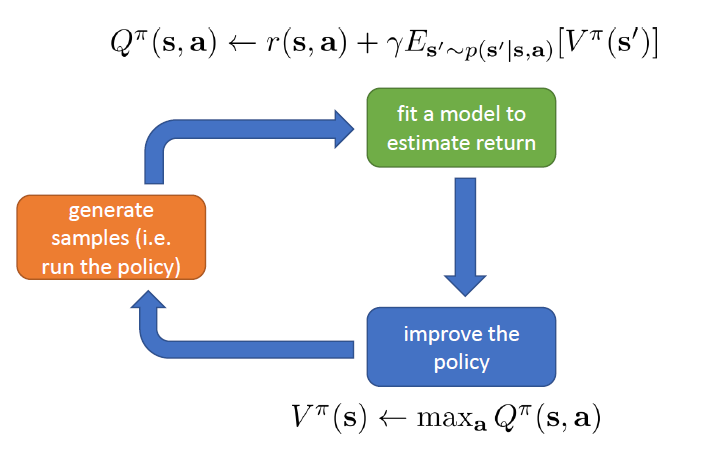
\includegraphics[width=\linewidth]{value-iter}
\caption{Value Iteration Algorithm}
\label{fig:value-iter}
\end{marginfigure}

\subsection{Q Iteration}

If we compute $Q^\pi (\s, \act)$ directly, it results in \emph{Q iteration algorithm} which is basically the same as \emph{value iteration algorithm} but with changing order of steps.

\begin{algorithm}
  \caption{Q Iteration Algorithm}
    \label{algo:q-iter}
    \begin{algorithmic}[1]
    % \REQUIRE some words.  % this command shows "Input"
    % \ENSURE
    \WHILE {\emph{Not converged}}
    \STATE Evaluate $ V^\pi (\s) = \max_\act Q(\s, \act)$. \\
    \STATE Update $Q^\pi (\s, \act) = r(\s, \act) +\gamma E[V^\pi(\s')]$. \\
    \ENDWHILE
    % \RETURN improved policy $\pi$  % this command shows "Output"
  \end{algorithmic}
\end{algorithm}

\section{Fitted Value Iteration}

How do we represent $V(s)$ in value iteration algorithm? For the discrete state space, we can do that with a big table, one entry for each state. But when the dimension of state space goes large, it's impractical \eg if the state is an image with size $200 \times 200$, the size of state space is
$ |\mathcal{S}| = (255^3)^ {200 \times 200}$ which is more than atoms in the universe. It's also referred as the \emph{curse of dimensionality}.

To deal with state space with large dimension, we can use approximator like neural network where the input is state $\s$, output is $V(\s)$, and weights of the network is denoted as $\phi$. As normal linear regression, we set the square distance as the loss function:

\begin{equation}
\label{eq:9}
\mathcal{L} (\phi) = \frac{1}{2} \bigg| \bigg| V_\phi (\s) - \max_\act Q^\pi(\s, \act) \bigg|\bigg| ^ 2
\end{equation}

We usually refer it as \emph{fitted value iteration algorithm}.

\begin{algorithm}

  \caption{Fitted Value Iteration Algorithm}
    \label{algo:fit-value}
    \begin{algorithmic}[1]
    % \REQUIRE some words.  % this command shows "Input"
    % \ENSURE
    \WHILE {\emph{Not converged}}
    \STATE Set $\mathbf{y}_i = \max_{\act_i} (r(\s_i, \act_i) +\gamma E[V_\phi(\s'_i)])$. \\
    \STATE Update $\phi = \arg \min_\phi 1/2 \sum_i || V_\phi(\s_i) - \mathbf{y}_i|| ^2 $. \\
    \ENDWHILE
    % \RETURN improved policy $\pi$  % this command shows "Output"
  \end{algorithmic}
\end{algorithm}

\begin{marginfigure}
\label{fig:v-net}
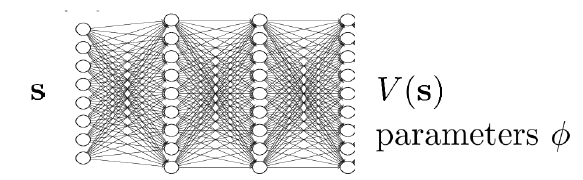
\includegraphics[width=\linewidth]{v-net}
\caption{Value function approximator}
\end{marginfigure}

When evaluating $\mathbf{y}_i$, it requires us to know the outcomes for different actions and we can do that with knowing dynamics or with sampling. But
it also requires us go back to the exact same previous step after going to the next state which is usually impractical.

\section{Fitted Q iteration}

What about approximating $Q^\pi(\s, \act)$ directly? From \emph{Q iteration}, if we approximate $E[V^\pi(\s')]$ with one sample of the next state:

\begin{equation}
\label{eq:10}
E[V^\pi(\s')] \approx \max_{\act'} Q(\s', \act')
\end{equation}

Then the resulting algorithms is referred as \emph{fitted Q iteration algorithm}.

\begin{algorithm}

  \caption{Fitted Q Iteration Algorithm}
    \label{algo:fit-q}
    \begin{algorithmic}[1]
    % \REQUIRE some words.  % this command shows "Input"
    % \ENSURE
    \WHILE {\emph{Not converged}}
    \STATE Approximate $E[V(\s'_i)]  \approx  \max_{\act'_i} Q_\phi(\s'_i, \act'_i)$. \\
    \STATE Set $\mathbf{y}_i = r(\s_i, \act_i) +\gamma E[V(\s'_i)]$. \\
    \STATE Update $\phi = \arg \min_\phi 1/2 \sum_i || Q_\phi(\s_i, \act_i) - \mathbf{y}_i|| ^2 $. \\
    \ENDWHILE
    % \RETURN improved policy $\pi$  % this command shows "Output"
  \end{algorithmic}
\end{algorithm}

\begin{marginfigure}
\label{fig:q-net}
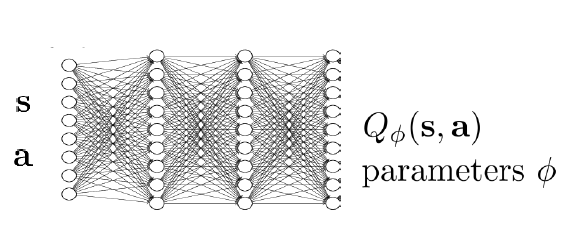
\includegraphics[width=\linewidth]{q-net}
\caption{Q-function approximator}
\end{marginfigure}

Where we can get rid of simulation of actions since the Q function tells the value for different actions. We still need the \emph{max} operation,
but it doesn't involve trying different actions in the real world, instead, we just need to try different actions in the function approximator.

It works even for off-policy \thanks{If the algorithm estimates the value function of the policy generating the data, the method is called on-policy.
Otherwise it is called off-policy.} samples and has one network with input as state and action, no high-variance policy gradient involved. However, there's no convergence guarantees for non-linear function approximation \thanks{We alluded this when discussing trade-off of different RL algorithms in lecture 2, and we will talk more about it later.}.

The fully fitted Q iteration algorithm including the data collecting phrase has many other options in practice.

\begin{algorithm}

  \caption{Fully Fitted Q Iteration Algorithm}
    \label{algo:full-fit-q}
    \begin{algorithmic}[1]
    % \REQUIRE some words.  % this command shows "Input"
    % \ENSURE
    \WHILE {\emph{Not converged}}
    \STATE Collect dataset $\{(\s_i, \act_i, \s'_i, r_i) \}$ using some policy. \\
      \WHILE {\emph{less than K steps}}
        \STATE Set $\mathbf{y}_i \approx r(\s_i, \act_i) +\gamma \max_{\act'_i} Q_\phi(\s'_i, \act'_i) $. \\
        \WHILE {\emph{less than S steps}}
          \STATE Update $\phi = \arg \min_\phi 1/2 \sum_i || Q_\phi(\s_i, \act_i) - \mathbf{y}_i|| ^2 $. \\
        \ENDWHILE
      \ENDWHILE
    \ENDWHILE
    % \RETURN improved policy $\pi$  % this command shows "Output"
  \end{algorithmic}
\end{algorithm}

Where K controls how further we choose to evaluate the Q-function and S controls how many iterations we take to improve the function approximator.

Why is this algorithm off-policy? In algorithm \ref{algo:full-fit-q}, $\max_{\act'_i} Q_\phi(\s'_i, \act'_i)$ estimates the value of the current policy
(optimal policy extracted from Q-function), and this estimation is valid regardless of where the state $\s'$ comes from, besides it updates with
$\arg \max$ in default even if the actual policy will not take the action that maximize Q function. It's like estimating the $Q(\s, \act)$ in the big table
of state-action space, what we are trying to do find out what the Q value is for each state-action pair regardless of where the state-action comes from.

It could be confusing what fitted Q iteration is trying to optimizing, cause the policy gradient is clear which heads to maximize the expected reward.
Actually, the fitted Q iteration minimizes the \emph{bellman error} $\mathcal{E}$.

\begin{equation}
\label{eq:11}
\mathcal{E} = \frac{1}{2} E_{(\s, \act) \sim \beta} \Big[Q_\phi(\s, \act) - [r(\s, \act) + \gamma \max_{\act'} Q_\phi (\s', \act')] \Big]
\end{equation}

Where the $(\s, \act)$ is distributed from the behavior policy $\beta$. if $\mathcal{E} = 0$, then

\begin{equation}
\label{eq:12}
Q_\phi(\s, \act)  = r(\s, \act) + \gamma \max_{\act'} Q_\phi (\s', \act')
\end{equation}

If the distribution $\beta$ has good coverage which assigns a probability to every possible state-action pair, then the Q function $Q_\phi(\s, \act)$
satisfies the equation \ref{eq:12} is called the optimal policy, corresponding to optimal policy $\pi'$ (following the mechanism in equation \ref{eq:13})

\begin{equation}
\label{eq:13}
\pi(\s_t | \act_t) =
\begin{cases}
1 \quad \text{if} \; \act_t = \arg \max_{\act_t} {Q}_\phi(\s_t, \act_t) \\
0 \quad \text{otherwise}
\end{cases}
\end{equation}

which leads to the maximized reward. However, when we leave the tabular case, these guarantees about the optimality are lost \eg using the neural network
function approximator.

\subsection{Online Q-learning}

We can change fitted Q-iteration into online version by taking only one step, and update Q once with one step of gradient descent.

\begin{algorithm}
  \caption{Online Q-learning Algorithm}
    \label{algo:online-q}
    \begin{algorithmic}[1]
    % \REQUIRE some words.  % this command shows "Input"
    % \ENSURE
    \WHILE {\emph{Not converged}}
    \STATE Take action $\act_i$ and observe $(\s_i, \act_i, \s'_i, r_i)$. \\
    \STATE Set $\mathbf{y}_i \approx r(\s_i, \act_i) +\gamma \max_{\act'_i} Q_\phi(\s'_i, \act'_i) $. \\
    \STATE Update $\phi \leftarrow \phi - \alpha \frac{d Q_\phi}{d \phi} (Q_\phi(\s_i, \act_i) - \mathbf{y}_i)$. \\
    \ENDWHILE
    % \RETURN improved policy $\pi$  % this command shows "Output"
  \end{algorithmic}
\end{algorithm}

But which action do we take for data collecting? One way is to follow our final policy, also referred as \emph{greedy policy} (equation \ref{eq:13}), but we might get stuck in some state which we think it's good and go to that state repeatedly without exploring other states. And this is a major problem in RL called \emph{exploration problem} into which we will dive deeper. Besides, exploration will has a great impact on range of support of the behavior
policy $\beta$. For now, we will introduce some methods with simple heuristics that people often choose to get around with the problem.

\textbf{Epsilon greedy}

The intuition is that the greedy policy is good but I will not fully commit to it, instead I will use a little factor $\epsilon$ to control the commitment, and do exploration with other actions with small probability.

\begin{equation}
\label{eq:14}
\pi(\act_t | \s_t) =
\begin{cases}
1- \epsilon \quad \text{if} \; \act_t = \arg \max_{\act_t} {Q}_\phi(\s_t, \act_t) \\
\epsilon/(|\mathcal{A}| -1) \quad \text{otherwise}
\end{cases}
\end{equation}

Where we think the other actions have equal probability and $\mathcal{A}$ is number of actions.

\textbf{Boltzmann exploration}

Another nuanced way is \emph{Boltzmann exploration}, intuitively, the Q function gives clue about which action is better or worse then we just follow it and construct probability of actions based on Q-function. Besides, we need the probabilities to be positive and normalized, then the exponent of Q-function
seems reasonably good.

\begin{equation}
\label{eq:15}
\pi(\act | \s) \propto \exp( Q_\phi (\s_t, \act_t))
\end{equation}

Later, we will find out that the Boltzmann exploration will lead to interesting connect between RL with probabilistic inference.

\section{Leaning theory}

We alluded that value based learning algorithms have no guarantees that it will converge to optimal policy when using function approximator, why is that?
And what about tabular case? Let's dive deeper to find out the mathematical explanation behind all of these.

Firstly, we define an operator $\mathcal{B}$:

\begin{equation}
\label{eq:16}
\mathcal{B}V = \max_\act r_\act + \gamma \mathcal{T}_\act V
\end{equation}

Where $r_\act$ is stacked vector of rewards at all states for action $\act$ \eg it's the element-wise maximization along horizontal axis in figure \ref{fig:tabular-q},
and $\mathcal{T}_\act$ is the matrix of transitions for action $\act$ such that $\mathcal{T}_{\act, i, j} = p(\s' = i | \s = j, \act)$.

We also define the \emph{fixed point} of $\mathcal{B}$ as $V^\star$ which satisfies:

\begin{equation}
\label{eq:17}
V^\star = \mathcal{B} V^\star = \max_\act r(\s, \act) + \gamma E[V^\star (\s')]
\end{equation}

In theory, the $V^\star$ always exists and is unique \thanks{TODO: prove it.}, besides it corresponds to the optimal policy.
We can prove that value iteration in \emph{tabular case} (algorithm \ref{algo:value-iter} which is the same as equation \ref{eq:17} mathematically) reaches $V^\star$ because
$\mathcal{B}$ is a \emph{contraction} \thanks{TODO: prove it} which means for any $V$ and $\bar{V}$, we have

\begin{equation}
\label{eq:18}
|| \mathcal{B}V - \mathcal{B} \bar{V} || _\infty \le \gamma || V - \bar{V} || _\infty
\end{equation}

After applying operator $\mathcal{B}$, the distance w.r.t to infinity norm gets small than that of before by discount factor $\gamma$. And if we choose
$V^\star$ as $\bar{V}$, we will converge eventually.

\begin{marginfigure}
\centering
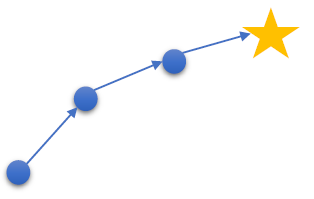
\includegraphics[width=\linewidth]{converge-b}
\caption{Illustration of value iteration convergence in tabular case}
\label{fig:conv-b}
\end{marginfigure}

For the non-tabular case \eg fitted value iteration algorithm (algorithm \ref{algo:fit-value}) which includes the regression step finding the function $V'$ which minimizes the squared error.

\begin{equation}
\label{eq:19}
V' \leftarrow \arg \min _{V' \in \Omega} \frac{1}{2} \sum \big | \big| V'(\s) - (\mathcal{B}V)(\s) \big|\big|^2
\end{equation}

Where $\Omega$ is the class of functions for the function approximator (\eg neural network). We can illustrate the update process with figure
\ref{fig:non-tab}. The plane represents all the possible functions, and the blue line means the possible function represented by current function approximator (\eg neural nets).
We start from function $V$ and applying operator $\mathcal{B}$ to jump off the manifold of $\Omega$, trying to reach the fixed point of $\mathcal{B}$.
Then with regression, we project $\mathcal{B}V$ back to $\Omega$ as $V'$ ideally.

\begin{marginfigure}
\centering
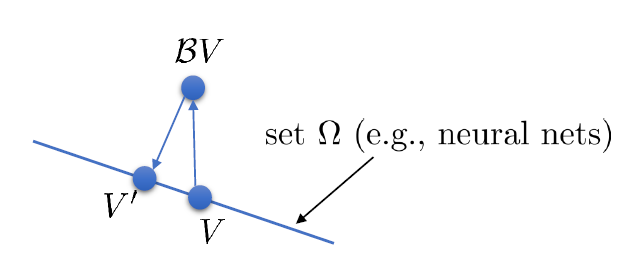
\includegraphics[width=\linewidth]{non-tab}
\caption{Illustration of updating process of fitted value iteration algorithm.}
\label{fig:non-tab}
\end{marginfigure}

Mathematically, we define a new operator $\Pi$:

\begin{equation}
\label{eq:20}
\Pi V = \arg \min _{V' \in \Omega} \frac{1}{2} \sum \big | \big| V'(\s) - (\mathcal{B}V)(\s) \big|\big|^2
\end{equation}

Where $\Pi$ is a \emph{projection} onto $\Omega$ in terms of $l_2$ norm. Then for fitted value iteration algorithm, we firstly apply \emph{back up} $\mathcal{B}$, then project it with $\Pi$:

\begin{equation}
\label{eq:21}
V \leftarrow \Pi \mathcal{B} V
\end{equation}

However the problem is that, the $\mathcal{B}$ is a contraction \wrt infinity norm ("max" norm), and $\Pi$ is a contraction \wrt $l_2$ norm (Euclidean distance), but $\Pi \mathcal{B}$ is not a contraction of any kind in general.

In a word, value iteration converges in tabular case and fitted value iteration does not converge in general. Besides, it also applies to Q-iteration algorithms.

\begin{marginfigure}
\centering
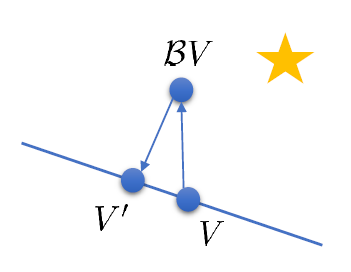
\includegraphics[width=\linewidth]{no-converge}
\caption{The star is the optimal function and learning procedure could drive away from the star in general.}
\label{fig:no-converge}
\end{marginfigure}

\end{document}
